%!TEX root = presentazionelancia.tex
\section{The Data Model}

\begin{frame}
\frametitle{Tao Data Model}
 	T.A.O. stands for ``The Associations and Objects"
 	\begin{center}
 	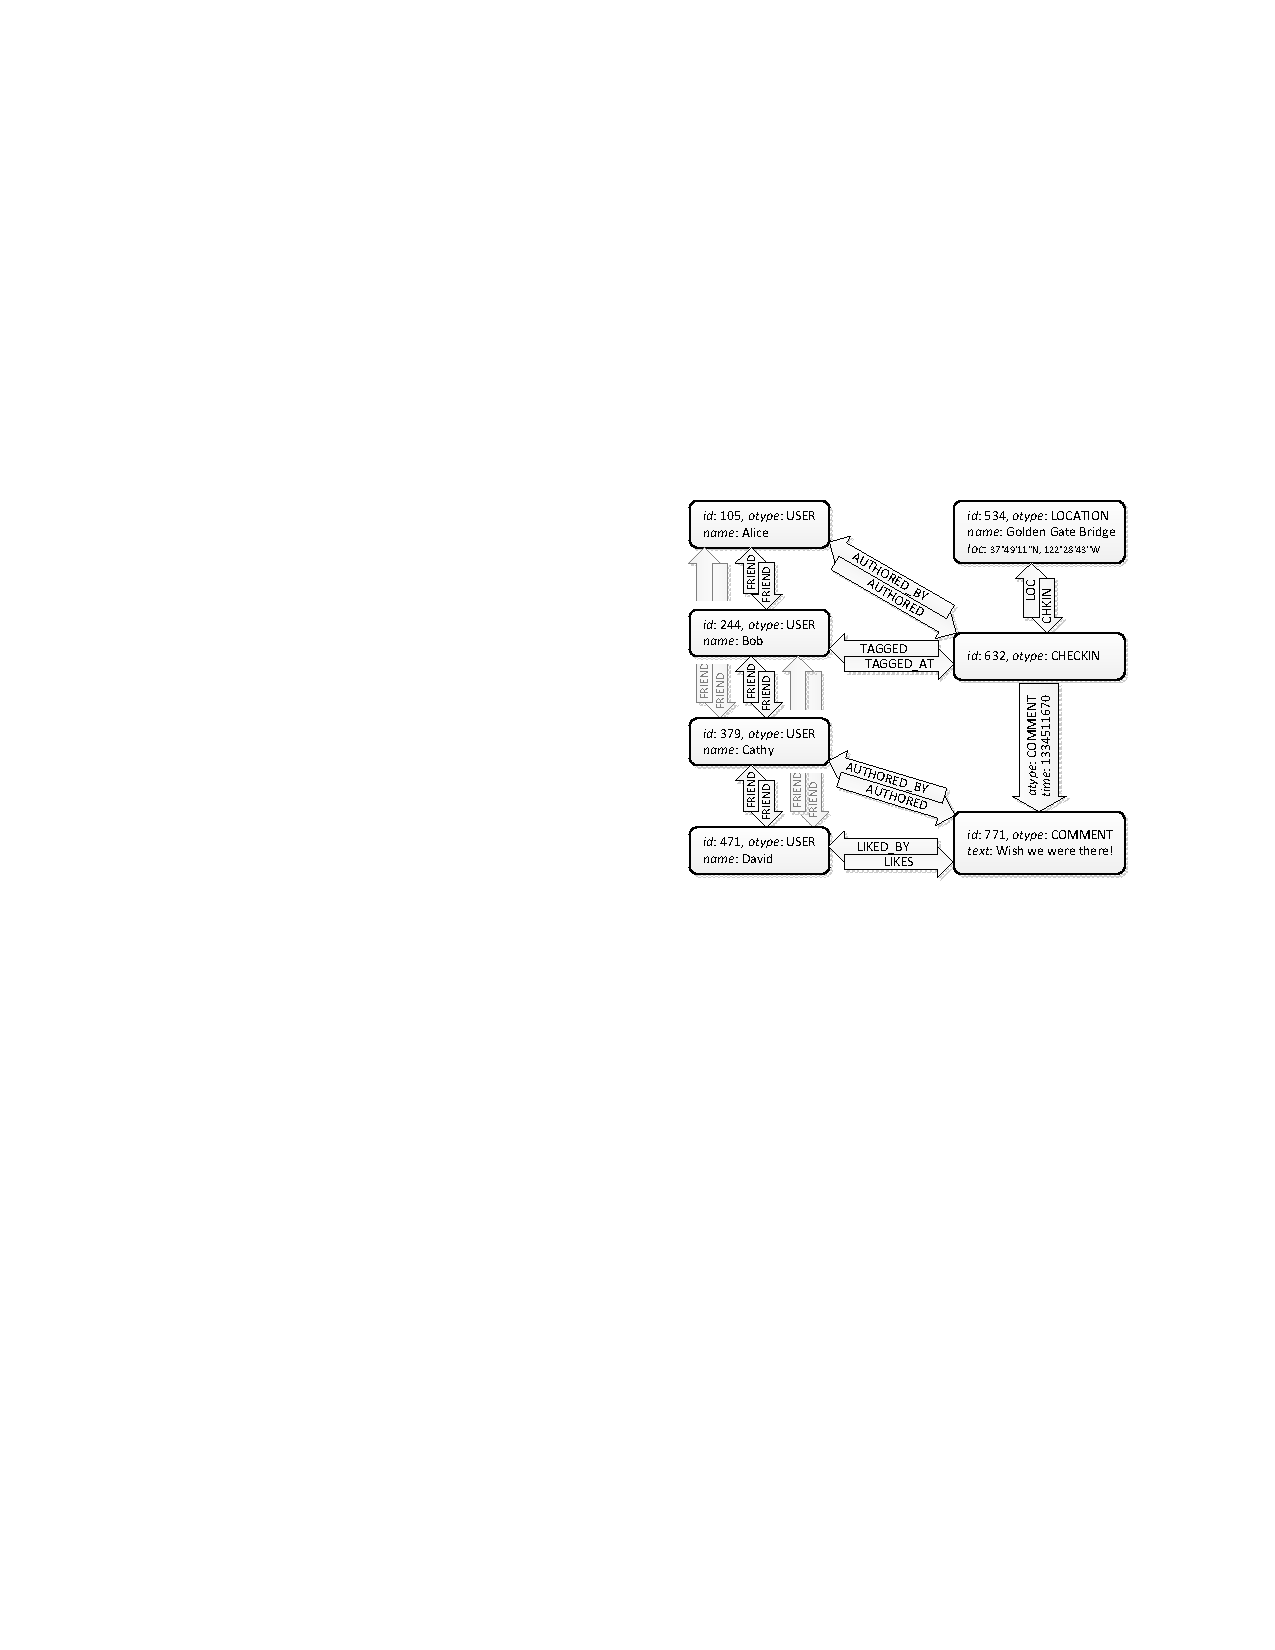
\includegraphics[width=0.6\textwidth]{figs/social2}		
 	\end{center}
\end{frame}

\begin{frame}[fragile]
\frametitle{Objects}
\onslide<1->
\begin{itemize}
	\item Typed nodes (type is denoted by \verb|otype|)
	\item Identified by 64-bit integers (unique) 
	\item Contains data in the form of key-value pairs
	\item Models users and repeatable actions (e.g. comments)
\end{itemize}
\onslide<2->
API for objects:
\begin{itemize}
	\item Allocate new object 
	\item retrieve
	\item update
	\item delete
\end{itemize}
 


\end{frame}


\begin{frame}
\frametitle{Associations}
    


\end{frame}